\subsection{Dynamics results}
\label{subsec:molecular_dynamics_results}

We start by looking into system evolution on a short time scale. For that we analyse time dependence of the order parameter~\eqref{eq:nematic_order_parameter} starting from different initial configurations outlined in previous section. The results for different densities are presented on the Figure~\ref{fig:short_time_order_parameter_different_density}. The squares stands for random initial configuration, the circles for co-aligned and triangles for counter-aligned initial configuration.

\begin{figure}[h]
\centering
\begin{subfigure}[t]{0.32\textwidth}
\begin{subfigure}[t]{\textwidth}
	\centering
	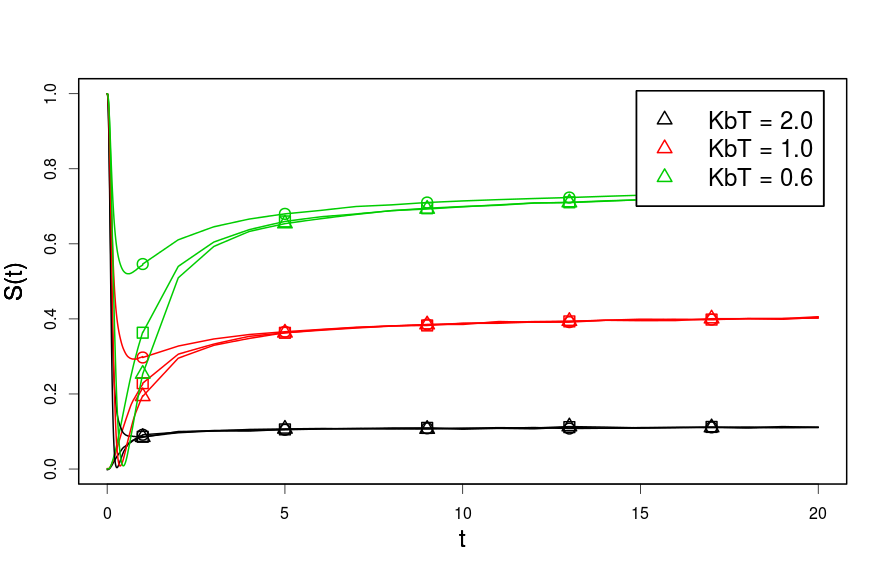
\includegraphics[width=\textwidth]{Images/op_relaxation_long_rho_05.png}
\end{subfigure}
\begin{subfigure}[t]{\textwidth}
	\centering
	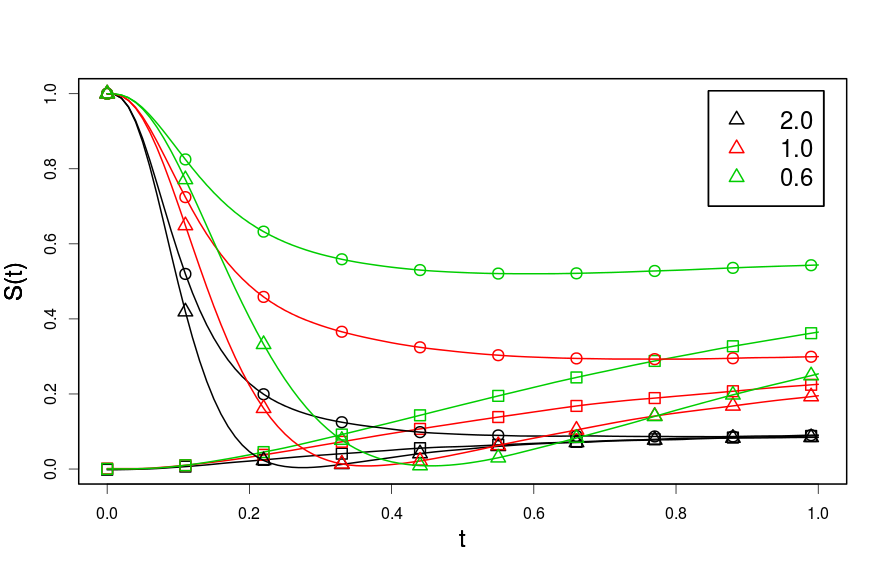
\includegraphics[width=\textwidth]{Images/op_relaxation_short_rho_05.png}
\end{subfigure}
	\captionsetup{justification=centering, width=0.9\columnwidth}
	\caption{$\rho = 0.5$}
\end{subfigure}
\begin{subfigure}[t]{0.32\textwidth}
\begin{subfigure}[t]{\textwidth}
	\centering
	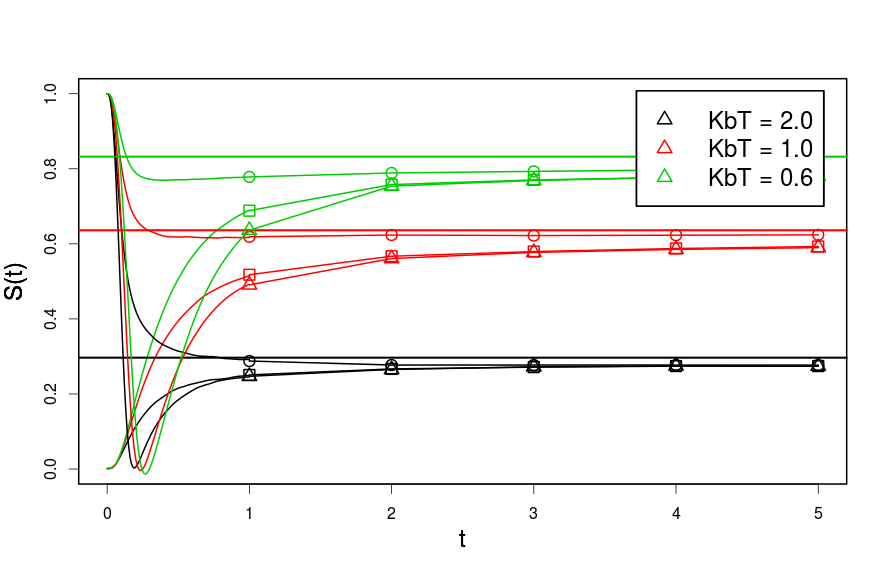
\includegraphics[width=\textwidth]{Images/op_relaxation_long_rho_075.png}
\end{subfigure}
\begin{subfigure}[t]{\textwidth}
	\centering
	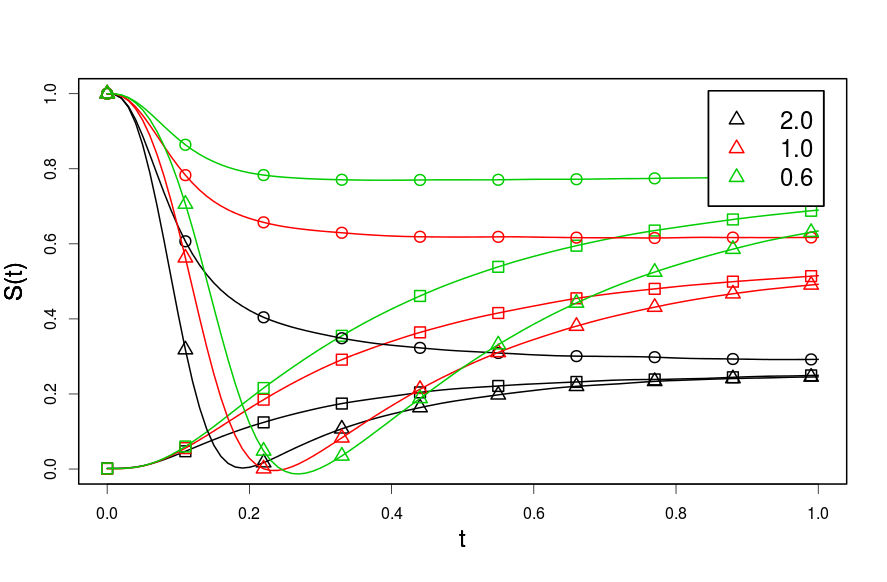
\includegraphics[width=\textwidth]{Images/op_relaxation_short_rho_075.png}
\end{subfigure}
	\captionsetup{justification=centering, width=0.9\columnwidth}
	\caption{$\rho = 0.75$}
\end{subfigure}
\begin{subfigure}[t]{0.32\textwidth}
\begin{subfigure}[t]{\textwidth}
	\centering
	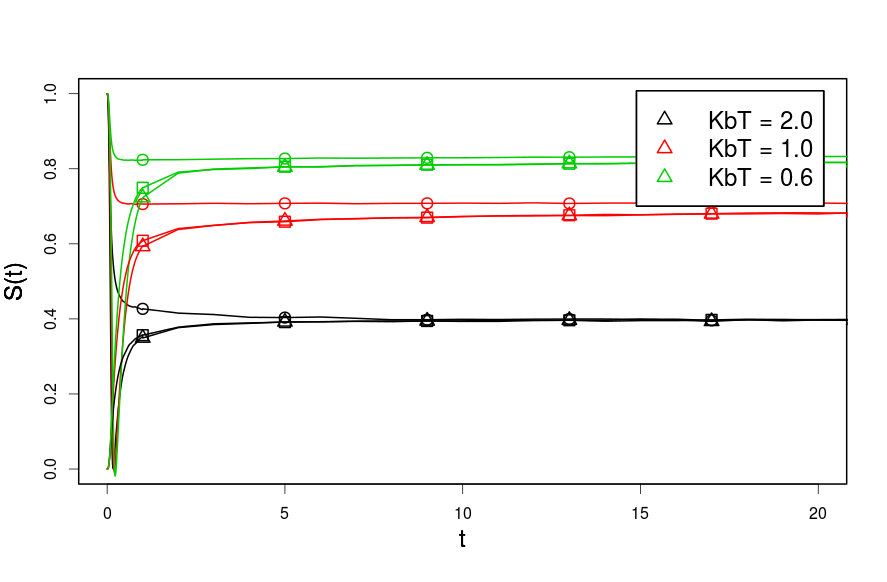
\includegraphics[width=\textwidth]{Images/op_relaxation_long_rho_085.png}
\end{subfigure}
\begin{subfigure}[t]{\textwidth}
	\centering
	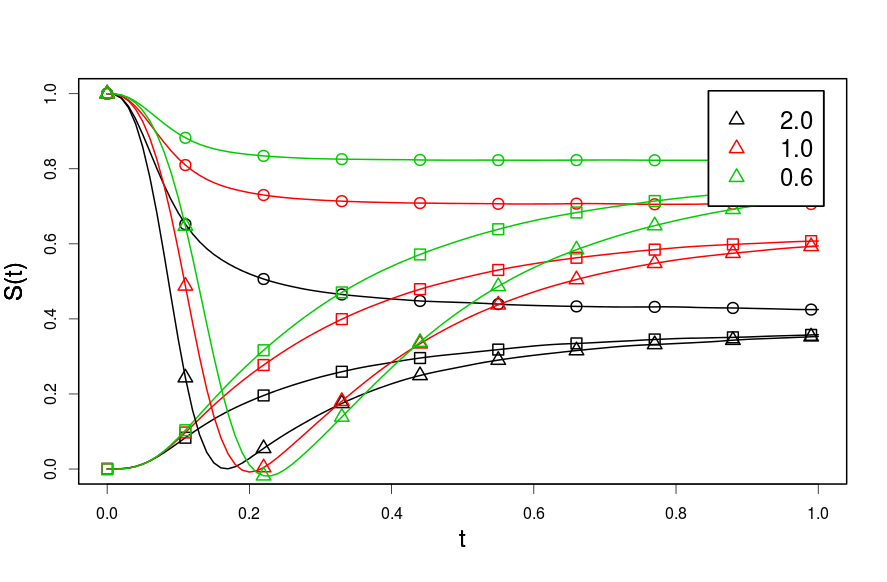
\includegraphics[width=\textwidth]{Images/op_relaxation_short_rho_085.png}
\end{subfigure}
	\captionsetup{justification=centering, width=0.9\columnwidth}
	\caption{$\rho = 0.85$}
\end{subfigure}
\captionsetup{justification=centering, width=0.9\columnwidth}
\caption{Order parameter as function of simulation time for different $k_BT$ and $\rho$. Squares indicates random initial configuration, circles --- co-aligned, and triangles --- counter-aligned. The simulations are performed for $N = 1600$ particles and the results are averaged over $100$ samples}
\label{fig:short_time_order_parameter_different_density}
\end{figure}

As we can see, for different density the influence of the initial configuration varies greatly. As expected, starting form the random configuration the order parameter starts growing and approaches the equilibrium results exponentially after some initial time. This behaviour is preserved for every value of density. If we start from counter-aligned initial configuration, the system rapidly relaxes to completely unaligned state, and after that it evolves the same way as the system with random initial configuration.

For the systems which starts from completely co-aligned configuration, however, the behaviour is more diverse. For sufficiently low density, the order parameter relaxes to the lower than the equilibrium value, and after some initial time the behaviour is the same as for randomly-oriented initial configuration. For high densities the order parameter relaxes directly to the equilibrium value.

\begin{figure}[h]
\centering
	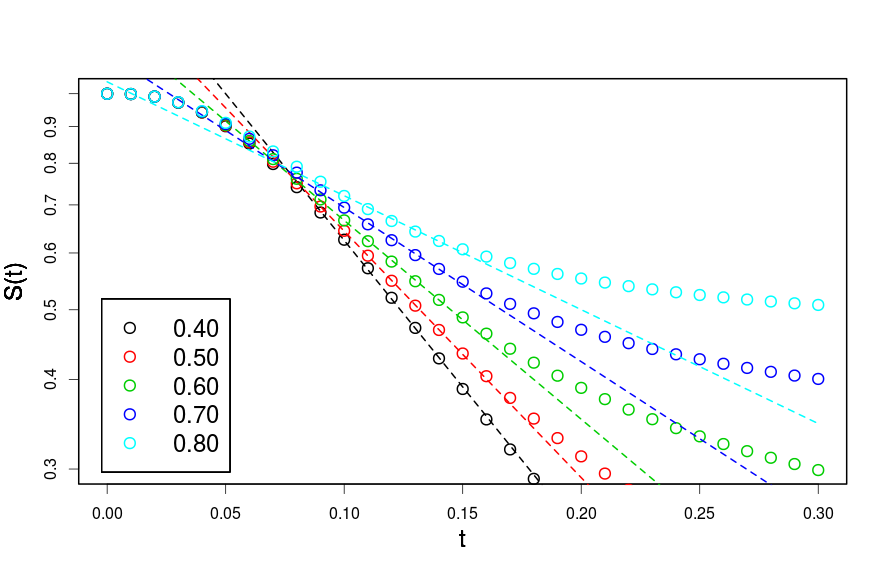
\includegraphics[width=0.5\textwidth]{Images/op_relaxation_short_fitting_kbt_1.png}
	\captionsetup{justification=centering, width=0.9\columnwidth}
	\caption{Order parameter as function of simulation time for different $\rho$ and one value of $k_BT = 1.6$. The simulations are performed for $N = 1600$ particles and the results are averaged over $100$ samples. Solid lines are the exponents fitted on the values from $t = 0.08$ to $t = 0.16$}
	\label{fig:short_time_order_parameter_fitting}
\end{figure}

As can be seen on the figure~\ref{fig:short_time_order_parameter_fitting} done in log-linear scale, the order parameter decays exponentially on the certain time period, which, in general, varies with density. \textcolor{red}{I believe that it varies linearly, but I don't know how to check that}. To better understand behaviour  of the system, we looked into the relations between short time exponent factors and $k_BT$ or $\rho$. It is clear from the figure~\ref{fig:exponential_factors:kbt}, that the short time exponential factors decays linearly with the increase of temperature for any given density. On the other hand, for any of the given $k_BT$, the density dependence of the short time exponent factors is more complicated. The function changes its curvature around the $\rho = 0.4$. For the densities higher than $0.4$ we supposed that short time exponential factors are proportional to $1/\rho^2$, so the dashed lines on the figure~\ref{fig:exponential_factors:rho} shows the least squared approximation \textcolor{red}{fitting} of the function of type $a/\rho^2 + b$ to the experimental values. \textcolor{red}{is there any physical predisposition to have exponential rather the power low dependance for low density? It fits slightly (like $10^{-6}$ lover least squared error) better than the power law} For the low density, however, it is equally. \textcolor{red}{The figure shows exponential fittings, and they are a tad better then power law, but well, it's to small}.

\begin{figure}[h]
\begin{subfigure}[t]{0.5\textwidth}
	\centering
	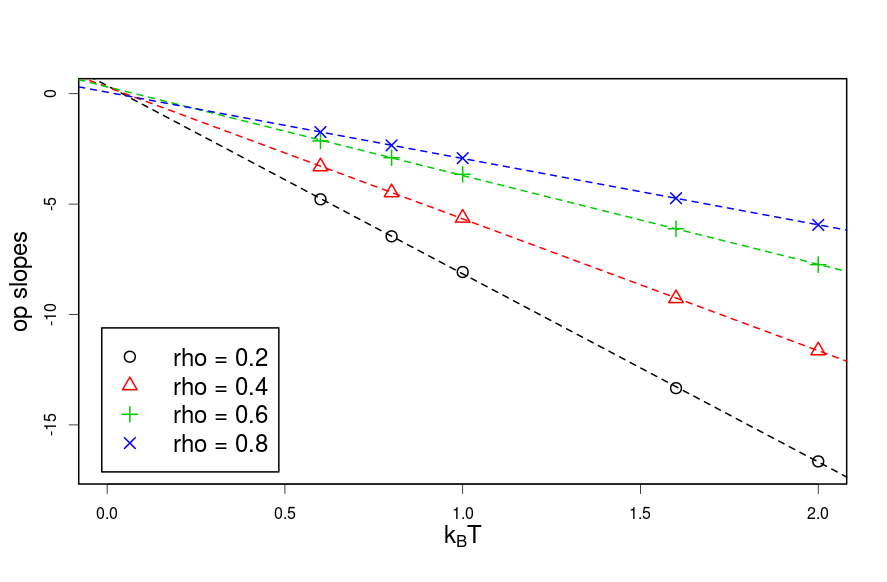
\includegraphics[width=\textwidth]{Images/op_slopes_short_vs_kbt.png}
	\captionsetup{justification=centering, width=0.9\columnwidth}
	\caption{}
	\label{fig:exponential_factors:kbt}
\end{subfigure}
\begin{subfigure}[t]{0.5\textwidth}
	\centering
	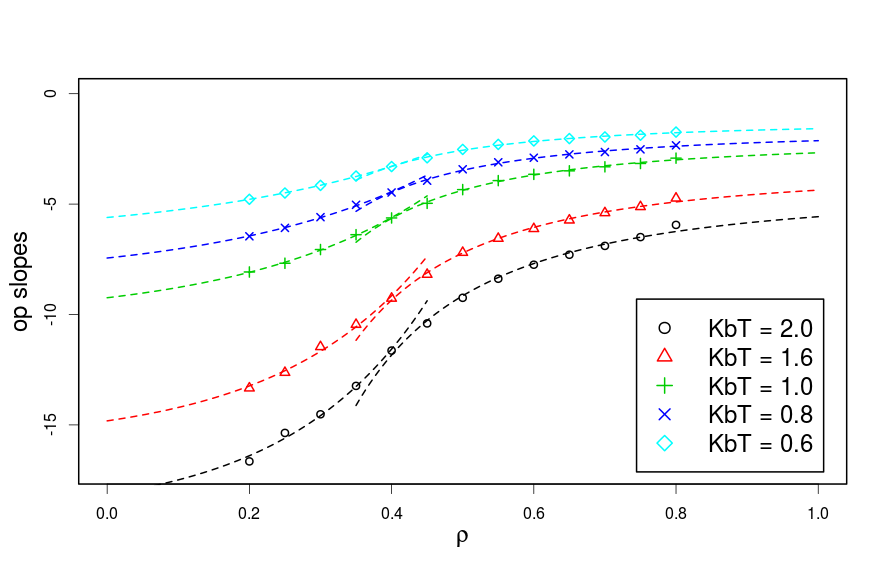
\includegraphics[width=\textwidth]{Images/op_slopes_short_vs_rho.png}
	\captionsetup{justification=centering, width=0.9\columnwidth}
	\caption{}
	\label{fig:exponential_factors:rho}
\end{subfigure}
\captionsetup{justification=centering, width=0.9\columnwidth}
\caption{Exponential factors of the order parameter as function of $k_BT$ (left) and $\rho$ (right) evaluated on the short time scale, starting from co-aligned configuration. The dotted lines are linear (left) and inverse squared $a/\rho^2$ (right for $\rho \geq 0.4$) and exponential (right for $\rho \leq 0.4$ functions best fitting the respective order parameter dependencies. As above, the results are averaged over $100$ samples.}
\label{fig:exponential_factors}
\end{figure}
